% Urutan cara kompilasi (command line) jika menggunakan XeLaTeX (berlaku juga untuk LaTeX, pdflatexmk, LuaLaTeX dll.)
%
% 1. xelatex ProposalTA.tex
% 2. biber ProposalTA      (tanpa .tex)
% 3. xelatex  ProposalTA.tex
% 4. xelatex  ProposalTA.tex
%
\documentclass[12pt,a4paper,oneside]{book}

% ==========================================
% PAKET DASAR
% ==========================================
\usepackage[utf8]{inputenc}
\usepackage{fontspec}
\setmainfont{Times New Roman}
\usepackage[a4paper, left=4cm, right=3cm, top=3cm, bottom=3cm]{geometry}
\usepackage[indonesian]{babel}
\usepackage{csquotes}
\usepackage{setspace}
\onehalfspacing
\usepackage{graphicx}
\usepackage{caption}
\usepackage{subcaption}
\usepackage{hyperref}
\usepackage{fancyhdr}
\usepackage{titlesec}
\usepackage{tocloft}
\usepackage{lipsum}
\usepackage{hyperref}
\usepackage{floatrow}

\setcounter{tocdepth}{4}
\setcounter{secnumdepth}{4}






% ==========================================
% SITASI DAN DAFTAR PUSTAKA (CHICAGO)
% ==========================================
\usepackage[
    backend=biber,
    authordate,
    language=english,
    autolang=other
]{biblatex-chicago}

\addbibresource{daftar-pustaka.bib}

% ==========================================
% Ubah istilah bahasa Inggris ke Bahasa Indonesia
% ==========================================
\DefineBibliographyStrings{english}{
  and          = {dan},
  andothers    = {dkk.},
  editor       = {penyunting},
  editors      = {penyunting},
  translator   = {penerjemah},
  byeditor     = {disunting oleh},
  bytranslator = {diterjemahkan oleh},
  in           = {dalam},
  edition      = {edisi},
  pages        = {hal.},
  page         = {hal.},
  volume       = {vol.},
  number       = {no.},
  urlseen      = {diakses pada},
  url          = {tautan},
}

% ==========================================
% Pastikan \cite() menampilkan (Penulis Tahun)
% ==========================================
\let\oldcite\cite
\renewcommand{\cite}{\parencite}

% ==========================================
% Atur pemisah nama penulis agar lebih natural dalam Bahasa Indonesia
% ==========================================
\renewcommand*{\finalandcomma}{} % hilangkan koma sebelum 'dan'


% ==========================================
% TAMPILAN
% ==========================================
\hypersetup{
    colorlinks=true,
    linkcolor=black,
    citecolor=black,
    urlcolor=black
}

%\fancyhf{}
%\fancyhead[R]{\thepage}
%\fancyhead[L]{\leftmark}
\pagestyle{plain}
%\renewcommand{\chaptermark}[1]{\markboth{\MakeUppercase{#1}}{}}
%\setlength{\parindent}{1.25cm}

% ==========================================
% AWAL DOKUMEN
% ==========================================
\begin{document}

% ==========================================
% HALAMAN JUDUL
% ==========================================
\begin{titlepage}
\begin{center}

    
    \vspace*{3cm}
    
    {\Large\bfseries PERANCANGAN SISTEM INFORMASI AKADEMIK BERBASIS WEB}\\
     \vspace{4cm}

    {\Large \textbf{Proposal Tugas Akhir}}\\


    \vspace{2cm}
    
    
    {\large Oleh}\\[0.3cm]
    \textbf{
    {\large John Doe}\\
    {\large 18299000}
    }\\

    \vspace{2cm}
    
    \begin{figure}[h]
    \centering
    
\includegraphics[width=0.2\textwidth]{ganesha.jpg}
    \end{figure}
    
    
     \vspace{1cm}

    \textbf{
    {\large PROGRAM STUDI SISTEM DAN TEKNOLOGI INFORMASI}\\
    {\large SEKOLAH TEKNIK ELEKTRO DAN INFORMATIKA}\\
    {\large INSTITUT TEKNOLOGI BANDUNG}\\
    {\large Desember 2025}
    }
\end{center}
\end{titlepage}



% ==========================================
% LEMBAR PENGESAHAN 
% ==========================================
\newpage
\thispagestyle{empty}
\pagenumbering{gobble}
\begin{center}
    \textbf{\large LEMBAR PENGESAHAN}\\[1cm]
    \vspace*{1.5cm}
    
    {\large\bfseries PERANCANGAN SISTEM INFORMASI AKADEMIK BERBASIS WEB}\\
     \vspace{2cm}

    {\Large \textbf{Proposal Tugas Akhir}}\\


    \vspace{1.5cm}
    
    
    {\large Oleh}\\[0.3cm]
    \textbf{
    {\large John Doe}\\
    {\large 18299000}
    }\\
    
 \vspace{0.5cm}
 
    {\large Program Studi Sistem dan Teknologi Informasi}\\
    {\large Sekolah Teknik Elektro dan Informatika}\\
    {\large Institut Teknologi Bandung}\\

 \vspace{1.5cm}

    Proposal Tugas Akhir ini telah disetujui dan disahkan\\ di Bandung, pada tanggal 20 November 2025\\[1cm]

% ==========================================
% Versi 1 pembimbing (default)
% ==========================================
	Pembimbing  \\[3cm]
	Dr. Ir. John Doe, M.T.   \\[0.2cm]
	NIP. 123456789 
% ==========================================

\end{center}

\vspace{1cm}
\noindent

% ==========================================
% Uncomment dan edit untuk versi 2 pembimbing
% ==========================================

%\begin{tabular}{p{1cm}p{7cm}p{7cm}}
%   & Pembimbing 1 & Pembimbing 2 \\[3cm]
%   & Dr. Ir. John Doe, M.T. & Dr. Mary Doe, M.Sc. \\[0.2cm]
%   &  NIP. 123456789 & NIP. 987654321
%\end{tabular}



% -- Change page number style to roman ---
\pagenumbering{roman} 


% ==========================================
% DAFTAR ISI, TABEL, GAMBAR
% ==========================================
% --- DAFTAR ISI ---
\makeatletter
\renewcommand{\tableofcontents}{%
  \clearpage
  \thispagestyle{plain}% no header
  \begin{center}
    {\large\bfseries\MakeUppercase{\contentsname}\par}
  \end{center}
  \vskip 1em
  \@starttoc{toc}%
}
\makeatother

\newpage
\renewcommand{\cfttoctitlefont}{\hfill\large\bfseries\MakeUppercase}
\renewcommand{\cftaftertoctitle}{\hfill}
\tableofcontents
\addcontentsline{toc}{chapter}{DAFTAR ISI}

% --- DAFTAR GAMBAR ---
\newpage
\renewcommand{\cftloftitlefont}{\hfill\large\bfseries\MakeUppercase}
\renewcommand{\cftafterloftitle}{\hfill}
\listoffigures
\addcontentsline{toc}{chapter}{DAFTAR GAMBAR}

% --- DAFTAR TABEL ---
\newpage
\renewcommand{\cftlottitlefont}{\hfill\large\bfseries\MakeUppercase}
\renewcommand{\cftafterlottitle}{\hfill}
\listoftables
\addcontentsline{toc}{chapter}{DAFTAR TABEL}




\mainmatter

\titleformat{\chapter}[display]
      {\centering\normalfont\large\bfseries} % Commands for the entire chapter title
      {\MakeUppercase \chaptertitlename\ \thechapter}{14pt}{\large} % Chapter number format

\titleformat{\section}
	{\normalfont\bfseries}
	{\thesection}{1em}{}
\titleformat{\subsection}
	{\normalfont\bfseries}
	{\thesubsection}{1em}{}

\setlength{\parindent}{0pt}
\renewcommand\thechapter{\Roman{chapter}}

\captionsetup[figure]{labelsep=space}
\captionsetup[table]{labelsep=space}
\floatsetup[table]{capposition=top}

\hypersetup{colorlinks=true, linkcolor=black}

% -- Change page number style to arabic ---
\pagenumbering{arabic} 
      
% ==========================================
% BAB I PENDAHULUAN
% ==========================================
\chapter{PENDAHULUAN}

% --- Latar Belakang ---
\section{Latar Belakang}
Latar Belakang menjelaskan dasar pemikiran, motivasi, kebutuhan, alasan, atau urgensi pemilihan masalah tugas akhir. Subbab ini berisi penjelasan ringkas tentang kondisi atau situasi yang ada saat ini terkait dengan topik yang dibahas. Tujuan utamanya adalah untuk memberikan informasi secukupnya kepada pembaca agar memahami topik yang akan dibahas. Dalam subbab ini, jelaskan hal-hal berikut ini:
\begin{enumerate}
\item	Kondisi atau situasi topik yang dibahas beserta permasalahannya, misalnya tentang pengelolaan informasi di puskesmas daerah pedesaan dan masalah yang dihadapi.
\item	Berbagai solusi yang telah diterapkan atau solusi yang tersedia dan memungkinkan untuk diterapkan untuk menyelesaikan masalah tersebut.
\end{enumerate}

% --- Rumusan Masalah ---
\section{Rumusan Masalah}
Rumusan Masalah berisi masalah utama yang dibahas dalam tugas akhir. Rumusan masalah yang baik memiliki struktur sebagai berikut:
\begin{enumerate}
\item	Pokok persoalan dari kondisi atau situasi yang ada saat ini. Dengan kata lain, jelaskan kelemahan atau kekurangan dari kondisi, situasi, atau solusi yang dijelaskan pada latar belakang. Ini merupakan pokok rumusan masalah.
\item	Elaborasi lebih lanjut urgensi penyelesaian masalah tersebut (mengapa penting untuk diselesaikan dan akibat yang dapat terjadi jika tidak diselesaikan).
\item	Usulan singkat terkait dengan solusi yang ditawarkan untuk menyelesaikan persoalan.
Penting untuk diperhatikan bahwa persoalan yang dideskripsikan pada subbab ini akan dipertanggungjawabkan di bab Evaluasi (apakah terselesaikan atau tidak).
\end{enumerate}

% --- Tujuan ---
\section{Tujuan}
Tuliskan tujuan utama dan/atau tujuan detail yang akan dicapai dalam pelaksanaan tugas akhir. Fokuskan pada hasil akhir yang ingin diperoleh setelah tugas akhir diselesaikan, terkait dengan penyelesaian persoalan pada rumusan masalah. Penting untuk diperhatikan bahwa tujuan yang dideskripsikan pada subbab ini akan dipertanggungjawabkan di akhir pelaksanaan tugas akhir apakah tercapai atau tidak. Tuliskan kriteria keberhasilan tugas akhir ini.

% --- Batasan Masalah ---
\section{Batasan Masalah}
Tuliskan batasan-batasan yang diambil dalam pelaksanaan tugas akhir. Batasan ini dapat dihindari (bersifat opsional, tidak perlu ada) jika topik atau judul tugas akhir dibuat cukup spesifik.

% --- Metodologi Pengerjaan TA ---
\section{Metodologi}
Tuliskan semua tahapan yang akan dilalui selama pelaksanaan tugas akhir. Tahapan ini spesifik untuk menyelesaikan persoalan tugas akhir. Khusus untuk penyusunan proposal ini, jelaskan secara detail:
\begin{enumerate}
\item	Tahapan investigasi pengumpulan fakta di latar belakang untuk merumuskan masalah.
\item	Langkah-langkah pencarian, pengelompokan, dan penapisan literatur atau sumber informasi untuk mengumpulkan informasi yang relevan tentang topik yang diangkat, termasuk teori (konsep atau teori apa saja yang perlu dicari), hal-hal yang telah dicapai oleh orang lain (cara mencari dan kata kuncinya), dan berbagai informasi pendukung, untuk mencari solusi terhadap masalah yang dibahas. Gunakan metodologi yang tepat dalam menggali informasi dan dokumentasikan prosesnya (termasuk rekaman wawancara atau survei) di dalam Lampiran, termasuk tautan ke video atau foto. Hasil penggalian informasi ini akan dijelaskan secara sistematis di Bab II Studi Literatur.
\end{enumerate}

% ==========================================
% BAB II STUDI LITERATUR
% ==========================================
\chapter{STUDI LITERATUR}
\section{Section Pertama}
\lipsum[1]
\subsection{Subsection Pertama}
\lipsum[2]
\subsubsection{Gambar}
Penomoran subbab maksimum adalah 4 (empat) tingkat, seperti pada nomor subbab ini. Contoh gambar dapat dilihat pada Gambar \ref{gambar:jaringan}. Gambar dan judulnya diposisikan di tengah. Nomor gambar tidak diakhiri tanda titik. Gambar tersebut dibuat menggunakan aplikasi draw.io dan disimpan ke format PNG setelah dengan zoom setting pada angka 300\%. Ukuran gambar yang ditampilkan dapat diatur dengan mengubah nilai \textit{width} dalam sintaks \textit{includegraphics}.

\begin{figure}[t] % pilihan opsi yang disarankan: t = top, b = bottom, h = here
	\centering
    	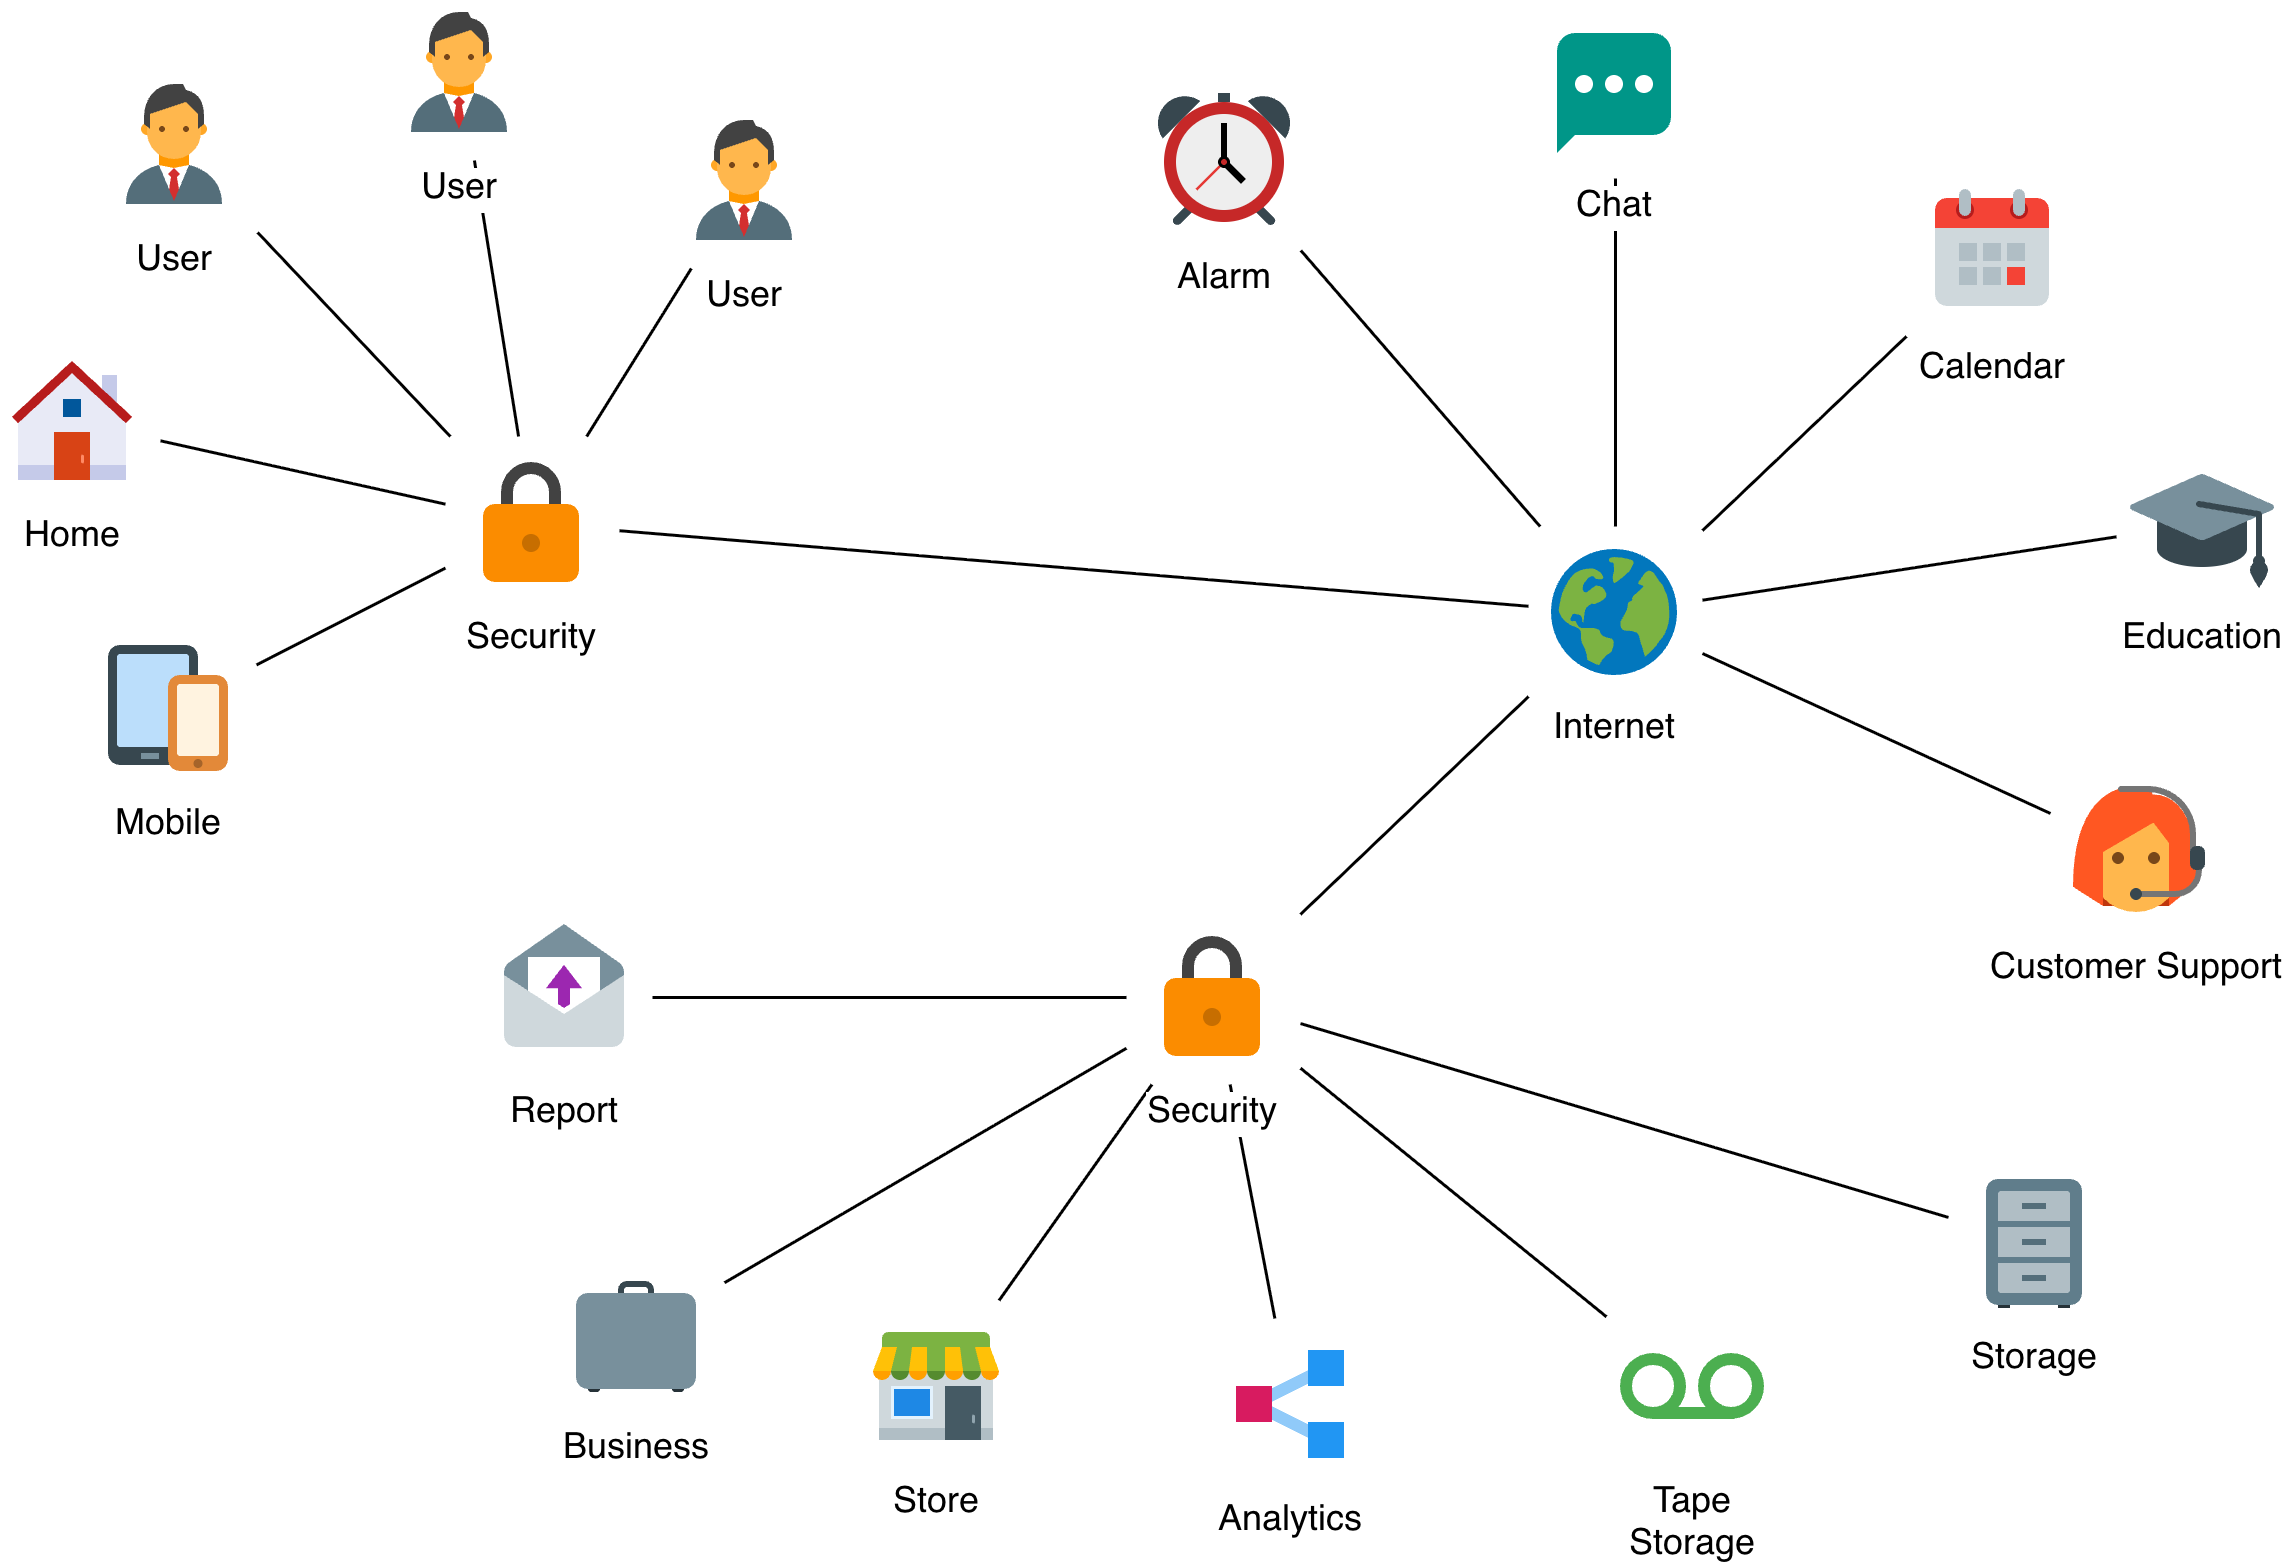
\includegraphics[width=0.5\textwidth]{gambar1.png}
	\caption{Contoh gambar jaringan}
	\label{gambar:jaringan}
\end{figure}


\subsubsection{Tabel}
Contoh tabel dapat dilihat pada Tabel \ref{tbl:harga1} dan \ref{tbl:harga2}. Tabel dan judulnya dibuat rata kiri dan judul tabel diletakkan di atas tabel. Usahakan tabel dapat ditulis dalam satu halaman, tidak terpotong ke halaman berikutnya.

\begin{table}[t] % pilihan opsi yang disarankan: t = top, b = bottom, h = here
\centering
	\begin{tabular}{ | p{2cm} | p{2cm} | p{3cm} |}
	\hline
	Nama 	& Satuan 		& Harga \\
	\hline
	Buku 	& Exemplar	& 25000 \\
	Komputer	& Unit		& 2500000 \\
	Pensil	& Buah		& 118900 \\
	\hline
	\end{tabular}
\caption{Tabel harga bahan pokok}
\label{tbl:harga1}
\end{table}

\begin{table}[h] % pilihan opsi yang disarankan: t = top, b = bottom, h = here
\centering
	\begin{tabular}{ | l | c | r | }
	\hline
	Nama 	& Satuan 		& Harga \\
	\hline
	Buku 	& Exemplar	& 25000 \\
	Komputer	& Unit		& 2500000 \\
	Pensil	& Buah		& 118900 \\
	\hline
	\end{tabular}
\caption{Tabel harga bahan sekunder}
\label{tbl:harga2}
\end{table}

\subsection{Subsection Kedua}
\lipsum[3]

% ==========================================
% BAB III ANALISIS MASALAH
% ==========================================
\chapter{ANALISIS MASALAH}
\section{Analisis Kondisi Saat Ini}
Menurut \textcite{laudon2020}, gambarkan terlebih dahulu model konseptual sistem yang ada saat ini. Model konseptual ini berisi berbagai komponen atau subsitem dan interaksi antarsubsistem tersebut. Setelah itu, berikan penjelasan tentang masalah yang ada pada sistem tersebut. Paragraf berikut berisi contoh penjabaran masalah sistem informasi fasilitas kesehatan untuk pasien \autocite{pressman2019}. 
\section{Analisis Kebutuhan}
\lipsum[1]

% ==========================================
% BAB IV DESAIN KONSEP SOLUSI
% ==========================================
\chapter{DESAIN KONSEP SOLUSI}
Bagian ini menjelaskan hasil implementasi dan evaluasi dari sistem informasi yang dirancang.

% ==========================================
% BAB V RENCANA SELANJUTNYA
% ==========================================
\chapter{RENCANA SELANJUTNYA}
Jelaskan secara detail langkah-langkah rencana selanjutnya, hal-hal yang diperlukan atau akan disiapkan, dan risiko dan mitigasinya, yang meliputi:
\begin{enumerate}
\item	Rencana implementasi, termasuk alat dan bahan yang diperlukan, lingkungan, konfigurasi, biaya, dan sebagainya.
\item	Desain pengujian dan evaluasi, misalnya metode verifikasi dan validasi.
\item	Analisis risiko dan mitigasi, misalnya tindakan selanjutnya jika ada yang tidak berjalan sesuai rencana.
\end{enumerate}


\backmatter

% ==========================================
% DAFTAR PUSTAKA
% ==========================================
\printbibliography[title={DAFTAR PUSTAKA}]

\appendix

\chapter{LAMPIRAN A: Source Code}


\chapter{LAMPIRAN B: Foto Lapangan}


\end{document}
 